% Overleaf compiler: pdfLaTeX. The bibliography uses BibTeX.
% Local build: latexmk -pdf General_Report_Template.tex
% Edit the BibTeX records below. LaTeX writes the .bib file at compile time.
\documentclass[12pt,a4paper]{report}

\begin{filecontents*}[overwrite]{btp_sample_references.bib}
@book{smith1997dsp,
  author    = {Smith, Steven W.},
  title     = {The Scientist and Engineer's Guide to Digital Signal Processing},
  publisher = {California Technical Publishing},
  year      = {1997},
  isbn      = {0-9660176-3-3}
}

@misc{nistMovingAverage,
  author       = {{NIST/SEMATECH}},
  title        = {Single Moving Average},
  howpublished = {\emph{e-Handbook of Statistical Methods}},
  note         = {Section 6.4.2.1.
                  \url{https://www.itl.nist.gov/div898/handbook/pmc/section4/pmc421.htm}}
}
\end{filecontents*}

\usepackage[margin=1in,headheight=15pt]{geometry}
\usepackage{setspace}
\usepackage{amsmath,amssymb}
\usepackage{graphicx}
\usepackage{booktabs}
\usepackage{fancyhdr}
\usepackage{pgfplots}
\usepackage[nottoc]{tocbibind}
\usepackage[hidelinks,hypertexnames=false]{hyperref}
\pgfplotsset{compat=1.18}

% Change these fields once to update the cover, certificate, and running headers.
\newcommand{\reportTitle}{Evaluating a Moving Average for Indoor Temperature Monitoring}
\newcommand{\reportType}{BTP Report (Sem-I)}
\newcommand{\authorName}{Name of Student}
\newcommand{\authorID}{XXXXXXXXX}
\newcommand{\supervisorName}{Name of supervisor}
\newcommand{\departmentName}{Mehta Family School of Data Science and Artificial Intelligence}
\newcommand{\institutionName}{Indian Institute of Technology Guwahati}
\newcommand{\reportDate}{November 2026}

% Change true to false to omit any of these front-matter pages.
\newif\ifshowCertificate
\showCertificatetrue
\newif\ifshowFigureList
\showFigureListtrue
\newif\ifshowTableList
\showTableListtrue

\onehalfspacing
\pagestyle{fancy}
\fancyhf{}
\fancyhead[L]{\small\itshape\reportType}
\fancyhead[R]{\small\itshape\authorName}
\fancyfoot[C]{\thepage}
\renewcommand{\headrulewidth}{0.4pt}
\renewcommand{\bibname}{References}

\begin{document}

\begin{titlepage}
  \centering
  \vspace*{2cm}
  
\includegraphics[width=4.4cm]{iit-guwahati-logo.png}\par
  \vspace{1.5cm}
  {\LARGE\bfseries\reportTitle\par}
  \vspace{0.8cm}
  {\large\reportType\par}
  \vspace{1.6cm}
  {\large\bfseries\authorName\par}
  Roll Number: \authorID\par
  \vfill
  {Submitted under the supervision of\par
   \large\bfseries\supervisorName\par}
  \vspace{1.2cm}
  \departmentName\par
  \institutionName\par
  \vspace{0.5cm}
  \reportDate\par
\end{titlepage}

\pagenumbering{roman}

\ifshowCertificate
  \chapter*{Certificate}
  \addcontentsline{toc}{chapter}{Certificate}
  % Replace this sample certificate with the wording your institution requires.
  This is to certify that \textbf{\authorName} (Roll Number: \authorID)
  completed the work presented in the report \emph{\reportTitle} under
  my supervision. The report was submitted to the \departmentName\
  at \institutionName.

  \vspace{2.5cm}
  \noindent Date: \rule{4cm}{0.4pt}\hfill
  \begin{minipage}[t]{0.45\textwidth}
    \rule{\linewidth}{0.4pt}\\
    \supervisorName\\
    Project Supervisor\\
    \departmentName
  \end{minipage}
\fi

\chapter*{Acknowledgements}
\addcontentsline{toc}{chapter}{Acknowledgements}

%I thank \supervisorName\ for guidance on defining the project scope,selecting evaluation metrics, and reviewing this report. I also thank my classmates for their feedback on how the results are presented.

\chapter*{Abstract}
\addcontentsline{toc}{chapter}{Abstract}

This sample project compares three approaches to displaying noisy indoor
temperature readings. We use ten synthetic observations with a known
two-degree change in the reference temperature. The raw readings are
compared with trailing moving averages of three and five observations.
On the six observations shared by all methods, the mean absolute error
is \(0.23\), \(0.39\), and \(0.67\,^{\circ}\mathrm{C}\), respectively.
The longer windows produce a slower response to the temperature change.
This example illustrates how to report an experiment, a quantitative
comparison, and the limits of the evidence.

\medskip
\noindent\textbf{Keywords.} Temperature monitoring, moving average,
time series, mean absolute error.

\tableofcontents
\ifshowFigureList
  \listoffigures
\fi
\ifshowTableList
  \listoftables
\fi

\clearpage
\pagenumbering{arabic}

\chapter{Introduction}

\section{Background and Motivation}

A temperature monitor reports a sequence of sensor readings over time.
Short fluctuations can make the display harder to interpret when the
room temperature is stable. Averaging recent readings is one way to
smooth the display, but it can also delay the response when the room
temperature changes.

\section{Problem Statement}

Given one temperature observation per minute, compare the raw readings
with two trailing moving averages. The comparison should show how
window length affects agreement with a known reference and how quickly
the display responds after a sudden change.

\section{Objectives}

\begin{enumerate}
  \item Implement trailing moving averages with three- and five-observation windows.
  \item Compare both windows against the raw readings using a shared evaluation interval.
  \item Quantify the trade-off between smoothing and response time.
\end{enumerate}

\chapter{Literature Review}

\section{Moving Averages for Smoothing}

A simple moving average uses equal weights for a fixed number of recent
observations \cite{nistMovingAverage}. Smith discusses the moving
average as a time-domain filter and describes the relationship between
window length, noise reduction, and step response \cite{smith1997dsp}.

\section{Scope of the Comparison}

This report uses a controlled temperature step to show how the filter
behaves when older observations come from a different temperature
level. The comparison uses a raw-reading baseline so that the effect
of adding a filter can be measured directly.

\chapter{Methodology}

\section{Sample Data}

The example uses ten synthetic temperature readings taken at one-minute
intervals. The reference is \(22\,^{\circ}\mathrm{C}\) for the first five
observations and \(24\,^{\circ}\mathrm{C}\) thereafter. The readings and
reference values are given in Appendix~\ref{app:data}.

\section{Filtering Method}

For observation \(x_t\) at index \(t\), the trailing average with window
length \(k\) is
\begin{equation}
  \widehat{x}^{(k)}_t = \frac{1}{k}\sum_{i=0}^{k-1} x_{t-i},
  \qquad t \geq k.
  \label{eq:moving-average}
\end{equation}
Equation~\eqref{eq:moving-average} uses the current and previous
observations, so it can be applied as new data arrive. The raw-reading
baseline corresponds to \(k=1\).

\section{Evaluation Metrics}

Mean absolute error (MAE) is the average of the absolute differences
between the reported and reference temperatures. All three methods
are evaluated over observations 5--10 because each window is fully
populated over this interval. Response delay is the time after
observation 6 until the output first lies within
\(0.25\,^{\circ}\mathrm{C}\) of the new reference temperature.

\chapter{Results and Discussion}

\section{Quantitative Results}

Table~\ref{tab:results} shows that the five-observation window has the
highest MAE and longest response delay in this example. The raw
readings enter the tolerance band at the first observation after the
change. The three-observation average enters the band two minutes later.

\begin{table}[htbp]
  \centering
  \caption{Performance on the synthetic temperature sequence.}
  \label{tab:results}
  \begin{tabular}{@{}lcc@{}}
    \toprule
    Method & MAE (\(^{\circ}\mathrm{C}\)) & Response delay (min) \\
    \midrule
    Raw readings (\(k=1\))    & 0.23 & 0 \\
    Moving average (\(k=3\))  & 0.39 & 2 \\
    Moving average (\(k=5\))  & 0.67 & 4 \\
    \bottomrule
  \end{tabular}
\end{table}

\section{Visual Comparison}

Figure~\ref{fig:temperature} shows why the longer window responds
slowly. Its first few estimates after the step still include readings
from the lower temperature period.

% This figure is generated from coordinates in LaTeX.
% For an external image, use \includegraphics[width=0.85\linewidth]{figure.png}.
\begin{figure}[htbp]
  \centering
  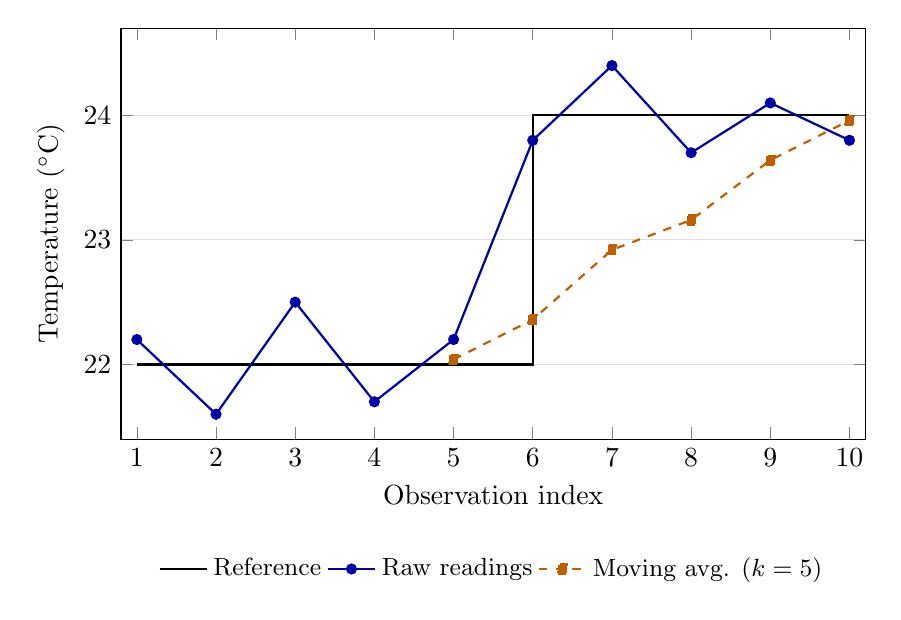
\begin{tikzpicture}
    \begin{axis}[
      width=0.91\linewidth,
      height=6.8cm,
      xlabel={Observation index},
      ylabel={Temperature (\(^{\circ}\mathrm{C}\))},
      xmin=0.8, xmax=10.2,
      ymin=21.4, ymax=24.7,
      xtick={1,2,3,4,5,6,7,8,9,10},
      ytick={22,23,24},
      ymajorgrids=true,
      grid style={gray!25},
      legend style={at={(0.5,-0.26)},anchor=north,draw=none,font=\small},
      legend columns=3,
    ]
      \addplot[black,thick,const plot] coordinates {
        (1,22) (2,22) (3,22) (4,22) (5,22)
        (6,24) (7,24) (8,24) (9,24) (10,24)
      };
      \addlegendentry{Reference}

      \addplot[blue!65!black,thick,mark=*,mark size=1.6pt] coordinates {
        (1,22.2) (2,21.6) (3,22.5) (4,21.7) (5,22.2)
        (6,23.8) (7,24.4) (8,23.7) (9,24.1) (10,23.8)
      };
      \addlegendentry{Raw readings}

      \addplot[orange!75!black,thick,dashed,mark=square*,mark size=1.6pt] coordinates {
        (5,22.04) (6,22.36) (7,22.92) (8,23.16) (9,23.64) (10,23.96)
      };
      \addlegendentry{Moving avg. (\(k=5\))}
    \end{axis}
  \end{tikzpicture}
  \caption{Reference temperature, raw readings, and five-observation
  moving average. The average begins at observation 5.}
  \label{fig:temperature}
\end{figure}

\section{Limitations}

The data are synthetic and contain one abrupt change. The aggregate MAE
therefore reflects this particular sequence and does not quantify
performance across different rooms, sensors, or noise conditions.

\chapter{Conclusion and Future Work}

\section{Conclusion}

The sample experiment shows how a longer moving-average window can
delay the response to an abrupt temperature change. For this sequence,
the raw readings achieved the lowest MAE, while the five-observation
window took four minutes to enter the tolerance band.

\section{Future Work}

A follow-up experiment could record multiple temperature transitions
from real sensors. It could report error separately during stable and
changing periods to distinguish steady-state smoothing from response delay.

% BibTeX uses the sample records defined at the top of this file.
\bibliographystyle{plain}
\bibliography{btp_sample_references}






\end{document}
